\subsection{Experimental Setup}

In the following, the performance of three localization algorithms is going to be compared:
the EKF-based localization  by Dantanarayana et al. \cite{Dantanarayana2016},
the EDH-based localization  algorithm proposed in this report,
and the Adaptive Monte Carlo Localization (AMCL) in ROS \cite{AMCLROS2002}.
For the sake of simplicity, the EDH-based, and the EKF-based
algorithms are going to be referred by their underlying filter (EDH and EKF).

To evaluate the algorithms, simulational data is provided by the Gazebo
simulator, where the TurtleBot3 robot is placed inside the TurtleBot3 House
(see Subsection \ref{subsec:robot} and \ref{subsec:map} for more details).

For one simulational run, the agent is driven around in the environment by hand.
Meanwhile, the AMCL runs in the background, and performs the localization.
The other two methods are not implemented in ROS, therefore require the
simulation data to be exported from Gazebo.
Upon the evaluation of the EKF and the EDH, this data is imported
from an external file, simulating real-time measurements.
This file contains the LiDAR measurements, the pose of the robot obtained
by odometry,
the ground truth pose, and the pose estimation by AMCL.

For AMCL, the default parameters are used, provided by ROBOTIS \footnote{https://github.com/ROBOTIS-GIT/turtlebot3}.
The initial mean of the EKF is the exact starting pose of the robot, and the
covariance is
\begin{equation}
    \boldsymbol\Sigma_0 = \text{diag}(\Sigma_{11},\Sigma_{22},\Sigma_{33}),
\end{equation}
where $\Sigma_{11} = 0.1^2\,\text{m}^2$,
$\Sigma_{22} = 0.1^2\,\text{m}^2$,$\Sigma_{33} = 0.05^2\,\text{rad}^2$.

The particles of the EDH are drawn from a prior with mean of the starting pose,
and covariance of $\boldsymbol\Sigma_0$.
For the homotopy, $N_\lambda$ = 10 steps are used, with $\Delta\lambda = 0.1$ as step size.

During different simulational runs, the particle number of the EDH,
and the odometry error constant $\kappa$ from \eqref{eq:odom-noise1} are varied.
\pagebreak
\subsection{Results}
Table \ref{tab:results}. contains the Root Mean Squared Error (RMSE) and Mean Absolute Error (MAE)
of the position and the orientation for different scenarios, using the ground truth pose data
from the simulator. The robustness of the algorithms are tested based on increasing odometry
noise by simulating with $\kappa = \{10^{-6},10^{-4},5\cdot10^{-3}\}$, producing three datasets.

For $\kappa = 10^{-4}$, the estimated trajectories by the filters are plotted in Figure \ref{fig:filtered-traj}.
(All three datasets have a similar ground truth path.) For this same simulation, the
estimation errors for each component of the pose are plotted
in Figures \ref{fig:setup2-x-error}-\ref{fig:setup2-th-error}.

By looking at these figures and the corresponding estimation errors in
Table \ref{tab:results} (rows 5-7), the superiority of the EKF and EDH based
localization algorithms are easily noticeable.
Moreover, the proposed EDH-based algorithm has the least amount of position error, and has only
slightly more orientation error than the EKF.
For less odometry noise ($\kappa = 10^6$), this difference disappears, and the three algorithm
produce similar results.

As $\kappa$ is increased, the position estimation advantage of the EDH algorithm becomes clearer,
although the EKF produces better orientation estimation. An important addition is that increasing
the particle number of the EDH does not yield a better result.

By comparing the estimation errors of the EKF and the EDH in Figure \ref{fig:setup2-x-error},
a beneficial property of the EDH is detectable.
Their error curves are broadly similar, but the EDH produces a less peaked
result, as it almost acts as a low-pass filter. The introduction of the log-homotopy,
and the averaging of the multiple tracked pose hypotheses (the particles)
are mainly responsible for this effect.

The main drawback of the AMCL algorithm lies in its poor performance of estimating
the orientation.  For $\kappa = 10^{-4}$, its position RMSE is twice than of the EDH,
but its orientation RMSE is 3.5 times higher.
Altogether, it is especially sensitive for the increasing odometry noise,
thus producing a 10 times higher RMSE than the EDH at $\kappa = 5\cdot10^{-3}$.

Generally, all of the algorithms performed well in the inspected scenarios, and
did not yield divergent results, even in the case of highly uncertain odometry data.
Inspecting the position errors, the EDH produced the lowest position errors in
all three runs, despite it only required 10 particles to do so.

Regarding computation time, the EKF took 0.52 s for a simulated movement of 429 s,
while the EDH took 40.4 s (running on an Apple M1 ARM with 8 GB of RAM
in Python 3.9).
Although this number is significantly higher
than in the case of the EKF, the main goal was the ability for the proposed
filter to be able to run in real time, which is fulfilled.
There are much room for improvement in in this field, as now the
subject of attention was on the realization of the proposed algorithm itself.
As the EDH operates with multiple particles, a significant improvement could
be achieved by the utilization of multiple CPU cores (making the computations
parallel).
\begin{figure}[htbp]
    \centering
    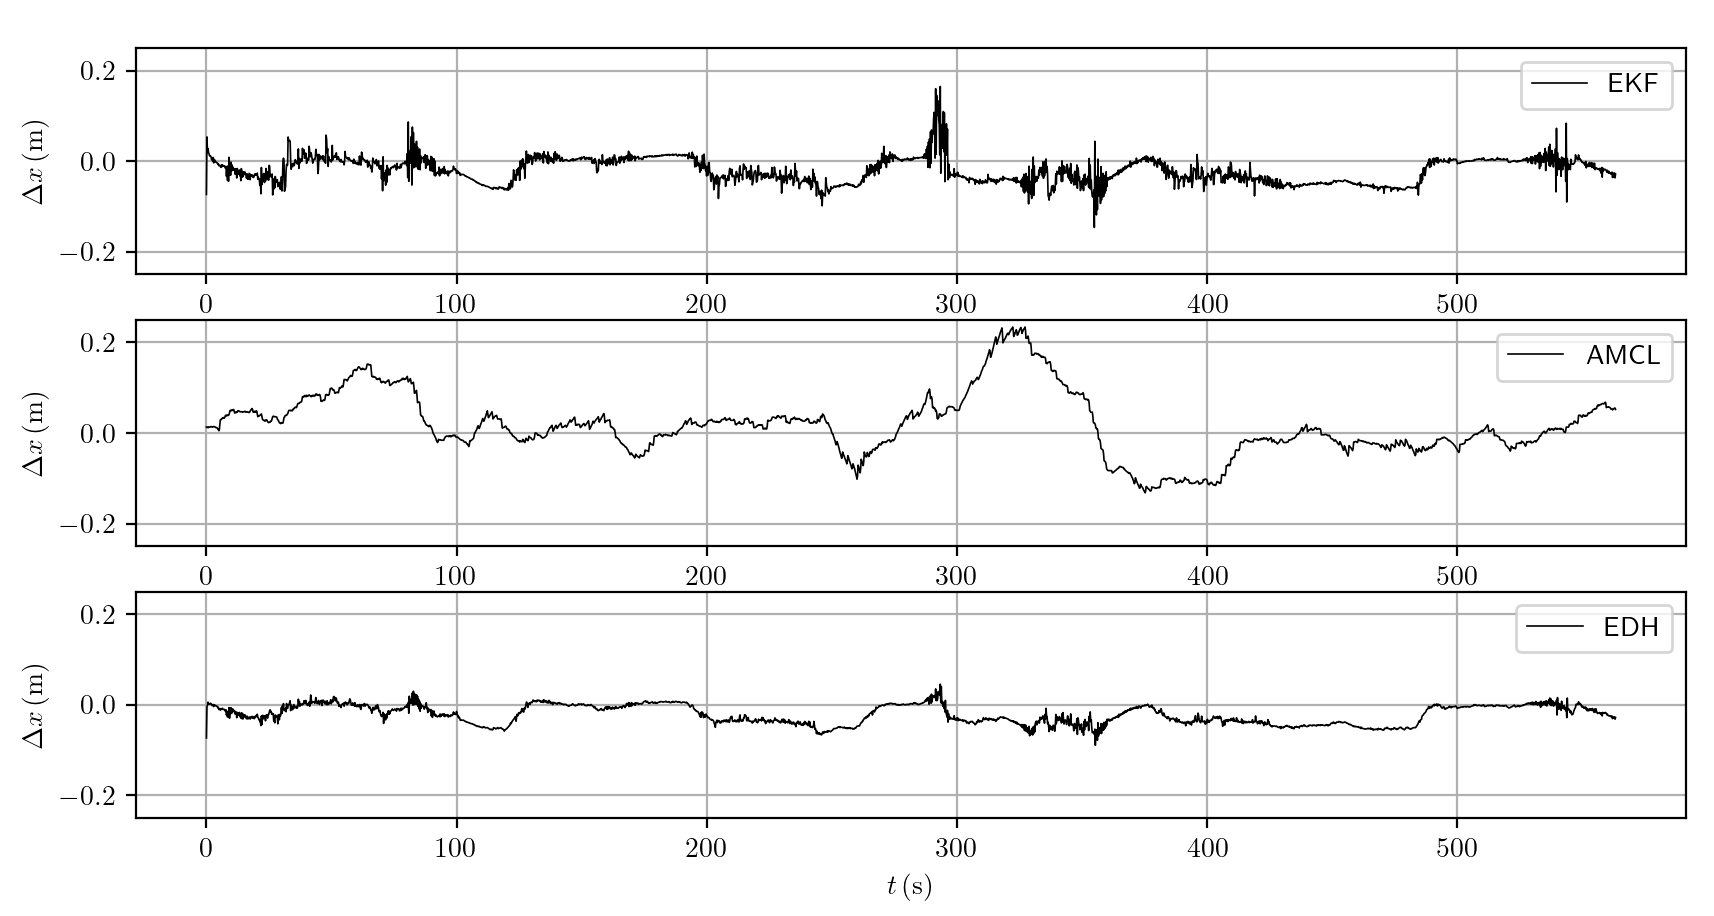
\includegraphics[width=\linewidth]{track_error_x.png}
    \caption{Position error against the ground truth in the $x$ component of the pose vector,
        using the dataset with $\kappa = 10^{-4}$.}
    \label{fig:setup2-x-error}
\end{figure}
\begin{figure}[htbp]
    \centering
    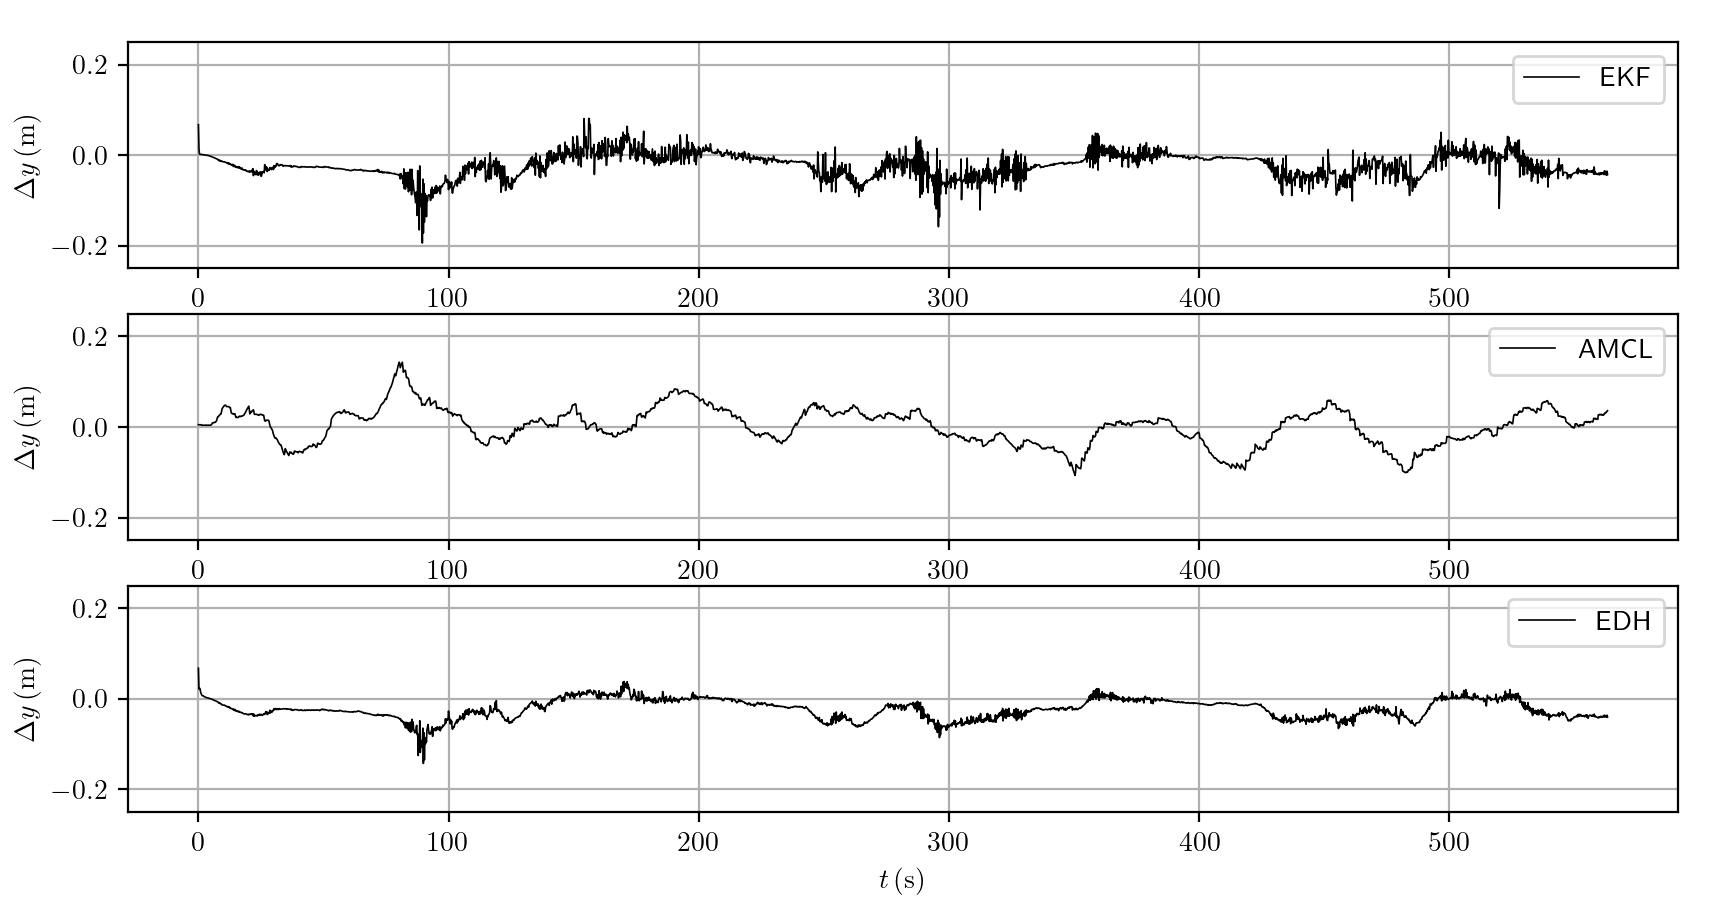
\includegraphics[width=\linewidth]{track_error_y.png}
    \caption{Position error against the ground truth in the $y$ component of the pose vector,
        using the dataset dataset with $\kappa = 10^{-4}$.}
    \label{fig:setup2-y-error}
\end{figure}
\begin{figure}[htbp]
    \centering
    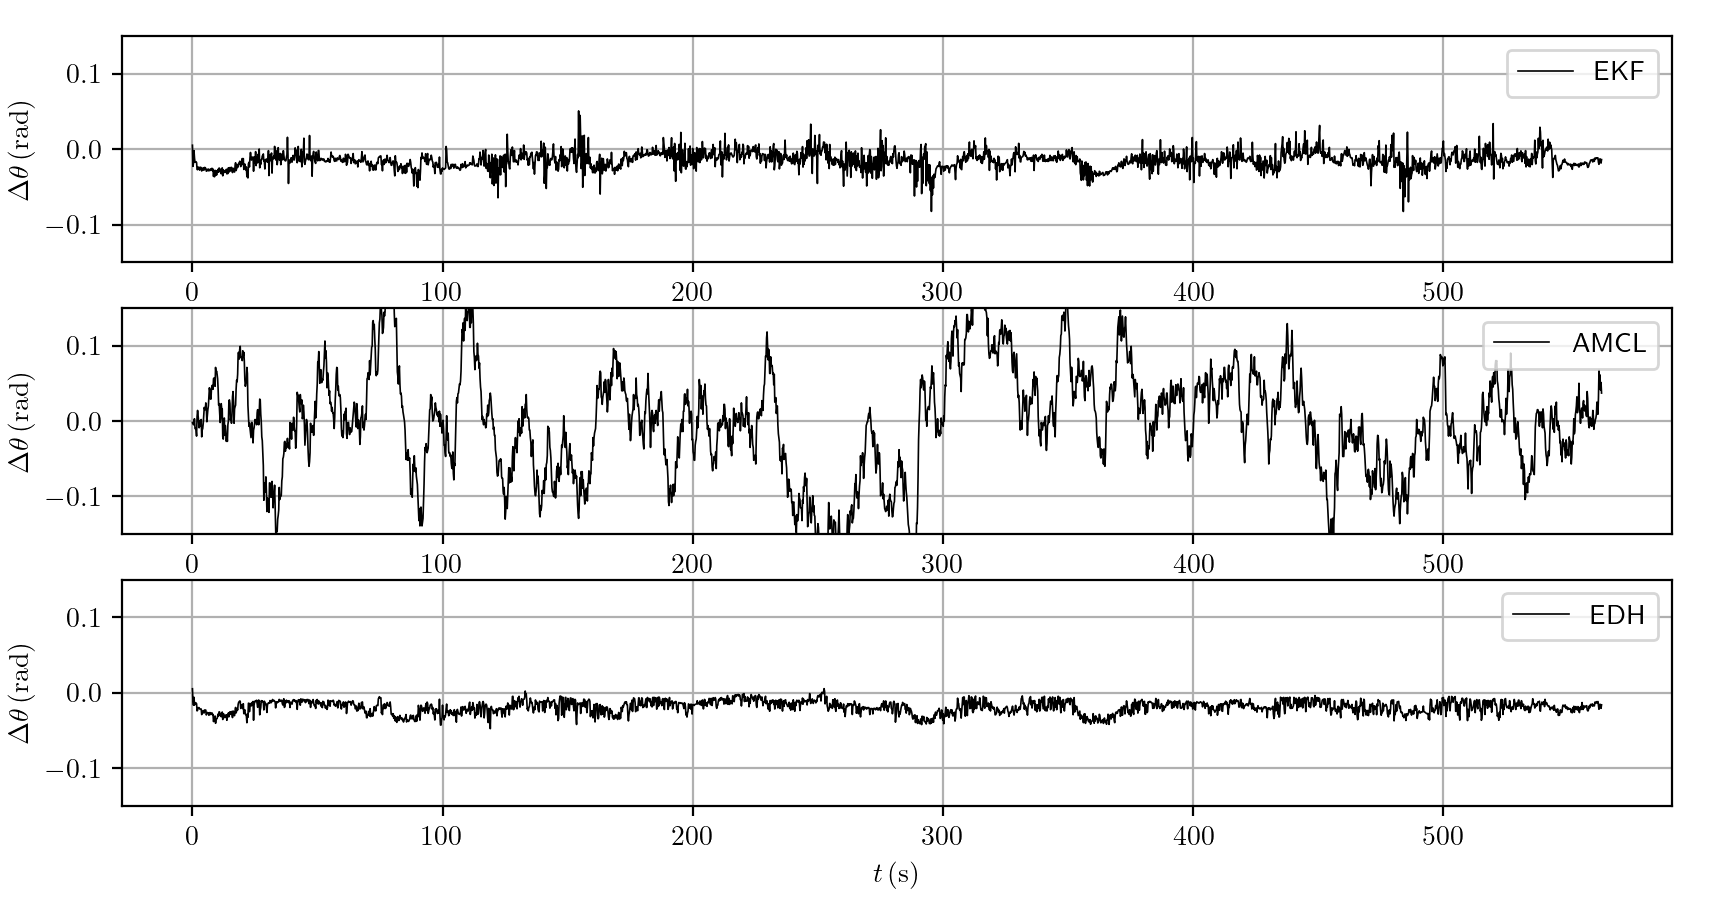
\includegraphics[width=\linewidth]{track_error_th.png}
    \caption{Orientation error against the ground truth in the $\theta$ component of the pose vector,
        using the  dataset with $\kappa = 10^{-4}$.}
    \label{fig:setup2-th-error}
\end{figure}
\begin{table}[]
    \centering
    \begin{tabular}{lllllll}
        \hline
        \multicolumn{1}{|c|}{\multirow{2}{*}{Algorithm}} & \multicolumn{1}{c|}{\multirow{2}{*}{\begin{tabular}[c]{@{}c@{}}$\kappa$\\(m)\end{tabular}}} & \multicolumn{1}{c|}{\multirow{2}{*}{\begin{tabular}[c]{@{}c@{}}Particle\\num.\end{tabular}}} & \multicolumn{2}{c|}{Root Mean Squared Error}   & \multicolumn{2}{c|}{Mean Absolute Error}                                                                                                          \\\cline{4-7}
        \multicolumn{1}{|c|}{}                           & \multicolumn{1}{c|}{}                                           & \multicolumn{1}{c|}{}                                           & \multicolumn{1}{l|}{\begin{tabular}[c]{@{}c@{}}position\\ (m)\end{tabular}} & \multicolumn{1}{c|}{\begin{tabular}[c]{@{}c@{}}orientation\\ (rad)\end{tabular}} & \multicolumn{1}{l|}{\begin{tabular}[c]{@{}c@{}}position\\ ($\text{m}$)\end{tabular}} & \multicolumn{1}{l|}{\begin{tabular}[c]{@{}c@{}}orientation\\ ($\text{rad}$)\end{tabular}} \\ \hline
        \hline
        \multicolumn{1}{|l|}{EKF}                        & \multicolumn{1}{c|}{$10^{-6}$}                                  & \multicolumn{1}{c|}{-}                                          & \multicolumn{1}{c|}{0.0559}                    & \multicolumn{1}{c|}{\textbf{0.0212}}           & \multicolumn{1}{c|}{0.0492}                    & \multicolumn{1}{c|}{\textbf{0.0168}}            \\ \hline
        \multicolumn{1}{|l|}{AMCL}                       & \multicolumn{1}{c|}{$10^{-6}$}                                  & \multicolumn{1}{c|}{adaptive}                                   & \multicolumn{1}{c|}{0.0529}                    & \multicolumn{1}{c|}{0.0233}                    & \multicolumn{1}{c|}{0.0453}                    & \multicolumn{1}{c|}{0.0177}                     \\ \hline
        \multicolumn{1}{|l|}{\multirow{3}{*}{EDH}}       & \multicolumn{1}{c|}{\multirow{3}{*}{$10^{-6}$}}                 & \multicolumn{1}{c|}{10}                                         & \multicolumn{1}{c|}{0.0504}                    & \multicolumn{1}{c|}{0.0228}                    & \multicolumn{1}{c|}{0.0449}                    & \multicolumn{1}{c|}{0.0183}                     \\ \cline{3-7}
        \multicolumn{1}{|l|}{}                           & \multicolumn{1}{c|}{}                                           & \multicolumn{1}{c|}{100}                                        & \multicolumn{1}{c|}{0.0504}                    & \multicolumn{1}{c|}{0.0229}                    & \multicolumn{1}{c|}{0.0447}                    & \multicolumn{1}{c|}{0.0183}                     \\ \cline{3-7}
        \multicolumn{1}{|l|}{}                           & \multicolumn{1}{c|}{}                                           & \multicolumn{1}{c|}{500}                                        & \multicolumn{1}{c|}{\textbf{0.0498}}           & \multicolumn{1}{c|}{0.0231}                    & \multicolumn{1}{c|}{\textbf{0.0441}}           & \multicolumn{1}{c|}{0.0185}                     \\ \hline
        \hline
        \multicolumn{1}{|l|}{EKF}                        & \multicolumn{1}{c|}{$10^{-4}$}                                  & \multicolumn{1}{c|}{-}                                          & \multicolumn{1}{c|}{0.0497}                    & \multicolumn{1}{c|}{\textbf{0.0186}}           & \multicolumn{1}{c|}{0.0428}                    & \multicolumn{1}{c|}{\textbf{0.0159}}            \\ \hline
        \multicolumn{1}{|l|}{AMCL}                       & \multicolumn{1}{c|}{$10^{-4}$}                                  & \multicolumn{1}{c|}{adaptive}                                   & \multicolumn{1}{c|}{0.0816}                    & \multicolumn{1}{c|}{0.0708}                    & \multicolumn{1}{c|}{0.0672}                    & \multicolumn{1}{c|}{0.0547}                     \\ \hline
        \multicolumn{1}{|l|}{\multirow{3}{*}{EDH}}       & \multicolumn{1}{c|}{\multirow{3}{*}{$10^{-4}$}}                 & \multicolumn{1}{c|}{10}                                         & \multicolumn{1}{c|}{0.0439}                    & \multicolumn{1}{c|}{0.0205}                    & \multicolumn{1}{c|}{\textbf{0.0381}}           & \multicolumn{1}{c|}{0.0188}                     \\ \cline{3-7}
        \multicolumn{1}{|l|}{}                           & \multicolumn{1}{c|}{}                                           & \multicolumn{1}{c|}{100}                                        & \multicolumn{1}{c|}{\textbf{0.0437}}           & \multicolumn{1}{c|}{0.0206}                    & \multicolumn{1}{c|}{0.0383}                    & \multicolumn{1}{c|}{0.0190}                     \\ \cline{3-7}
        \multicolumn{1}{|l|}{}                           & \multicolumn{1}{c|}{}                                           & \multicolumn{1}{c|}{500}                                        & \multicolumn{1}{c|}{0.0438}                    & \multicolumn{1}{c|}{0.0206}                    & \multicolumn{1}{c|}{0.0382}                    & \multicolumn{1}{c|}{0.0190}                     \\ \hline
        \hline
        \multicolumn{1}{|l|}{EKF}                        & \multicolumn{1}{c|}{$5\cdot10^{-3}$}                            & \multicolumn{1}{c|}{-}                                          & \multicolumn{1}{c|}{0.0732}                    & \multicolumn{1}{c|}{\textbf{0.0297}}           & \multicolumn{1}{c|}{0.0610}                    & \multicolumn{1}{c|}{\textbf{0.0256}}            \\ \hline
        \multicolumn{1}{|l|}{AMCL}                       & \multicolumn{1}{c|}{$5\cdot10^{-3}$}                            & \multicolumn{1}{c|}{adaptive}                                   & \multicolumn{1}{c|}{0.5261}                    & \multicolumn{1}{c|}{0.4940}                    & \multicolumn{1}{c|}{0.3533}                    & \multicolumn{1}{c|}{0.3841}                     \\ \hline
        \multicolumn{1}{|l|}{\multirow{3}{*}{EDH}}       & \multicolumn{1}{c|}{\multirow{3}{*}{$5\cdot10^{-3}$}}           & \multicolumn{1}{c|}{10}                                         & \multicolumn{1}{c|}{\textbf{0.0587}}           & \multicolumn{1}{c|}{0.0401}                    & \multicolumn{1}{c|}{\textbf{0.0494}}           & \multicolumn{1}{c|}{0.0372}                     \\ \cline{3-7}
        \multicolumn{1}{|l|}{}                           & \multicolumn{1}{c|}{}                                           & \multicolumn{1}{c|}{100}                                        & \multicolumn{1}{c|}{0.0616}                    & \multicolumn{1}{c|}{0.0403}                    & \multicolumn{1}{c|}{0.0503}                    & \multicolumn{1}{c|}{0.0374}                     \\ \cline{3-7}
        \multicolumn{1}{|l|}{}                           & \multicolumn{1}{c|}{}                                           & \multicolumn{1}{c|}{500}                                        & \multicolumn{1}{c|}{0.0617}                    & \multicolumn{1}{c|}{0.0402}                    & \multicolumn{1}{c|}{0.0503}                    & \multicolumn{1}{c|}{0.0373}                     \\ \hline
        \hline
    \end{tabular}
    \caption{Estimation errors of the three filters on three distinct dataset, with increasing odometry error $\kappa$.
        The best results are indicated by bold font for each dataset and each category.}
    \label{tab:results}
\end{table}

\begin{figure}[htbp]
    \centering
    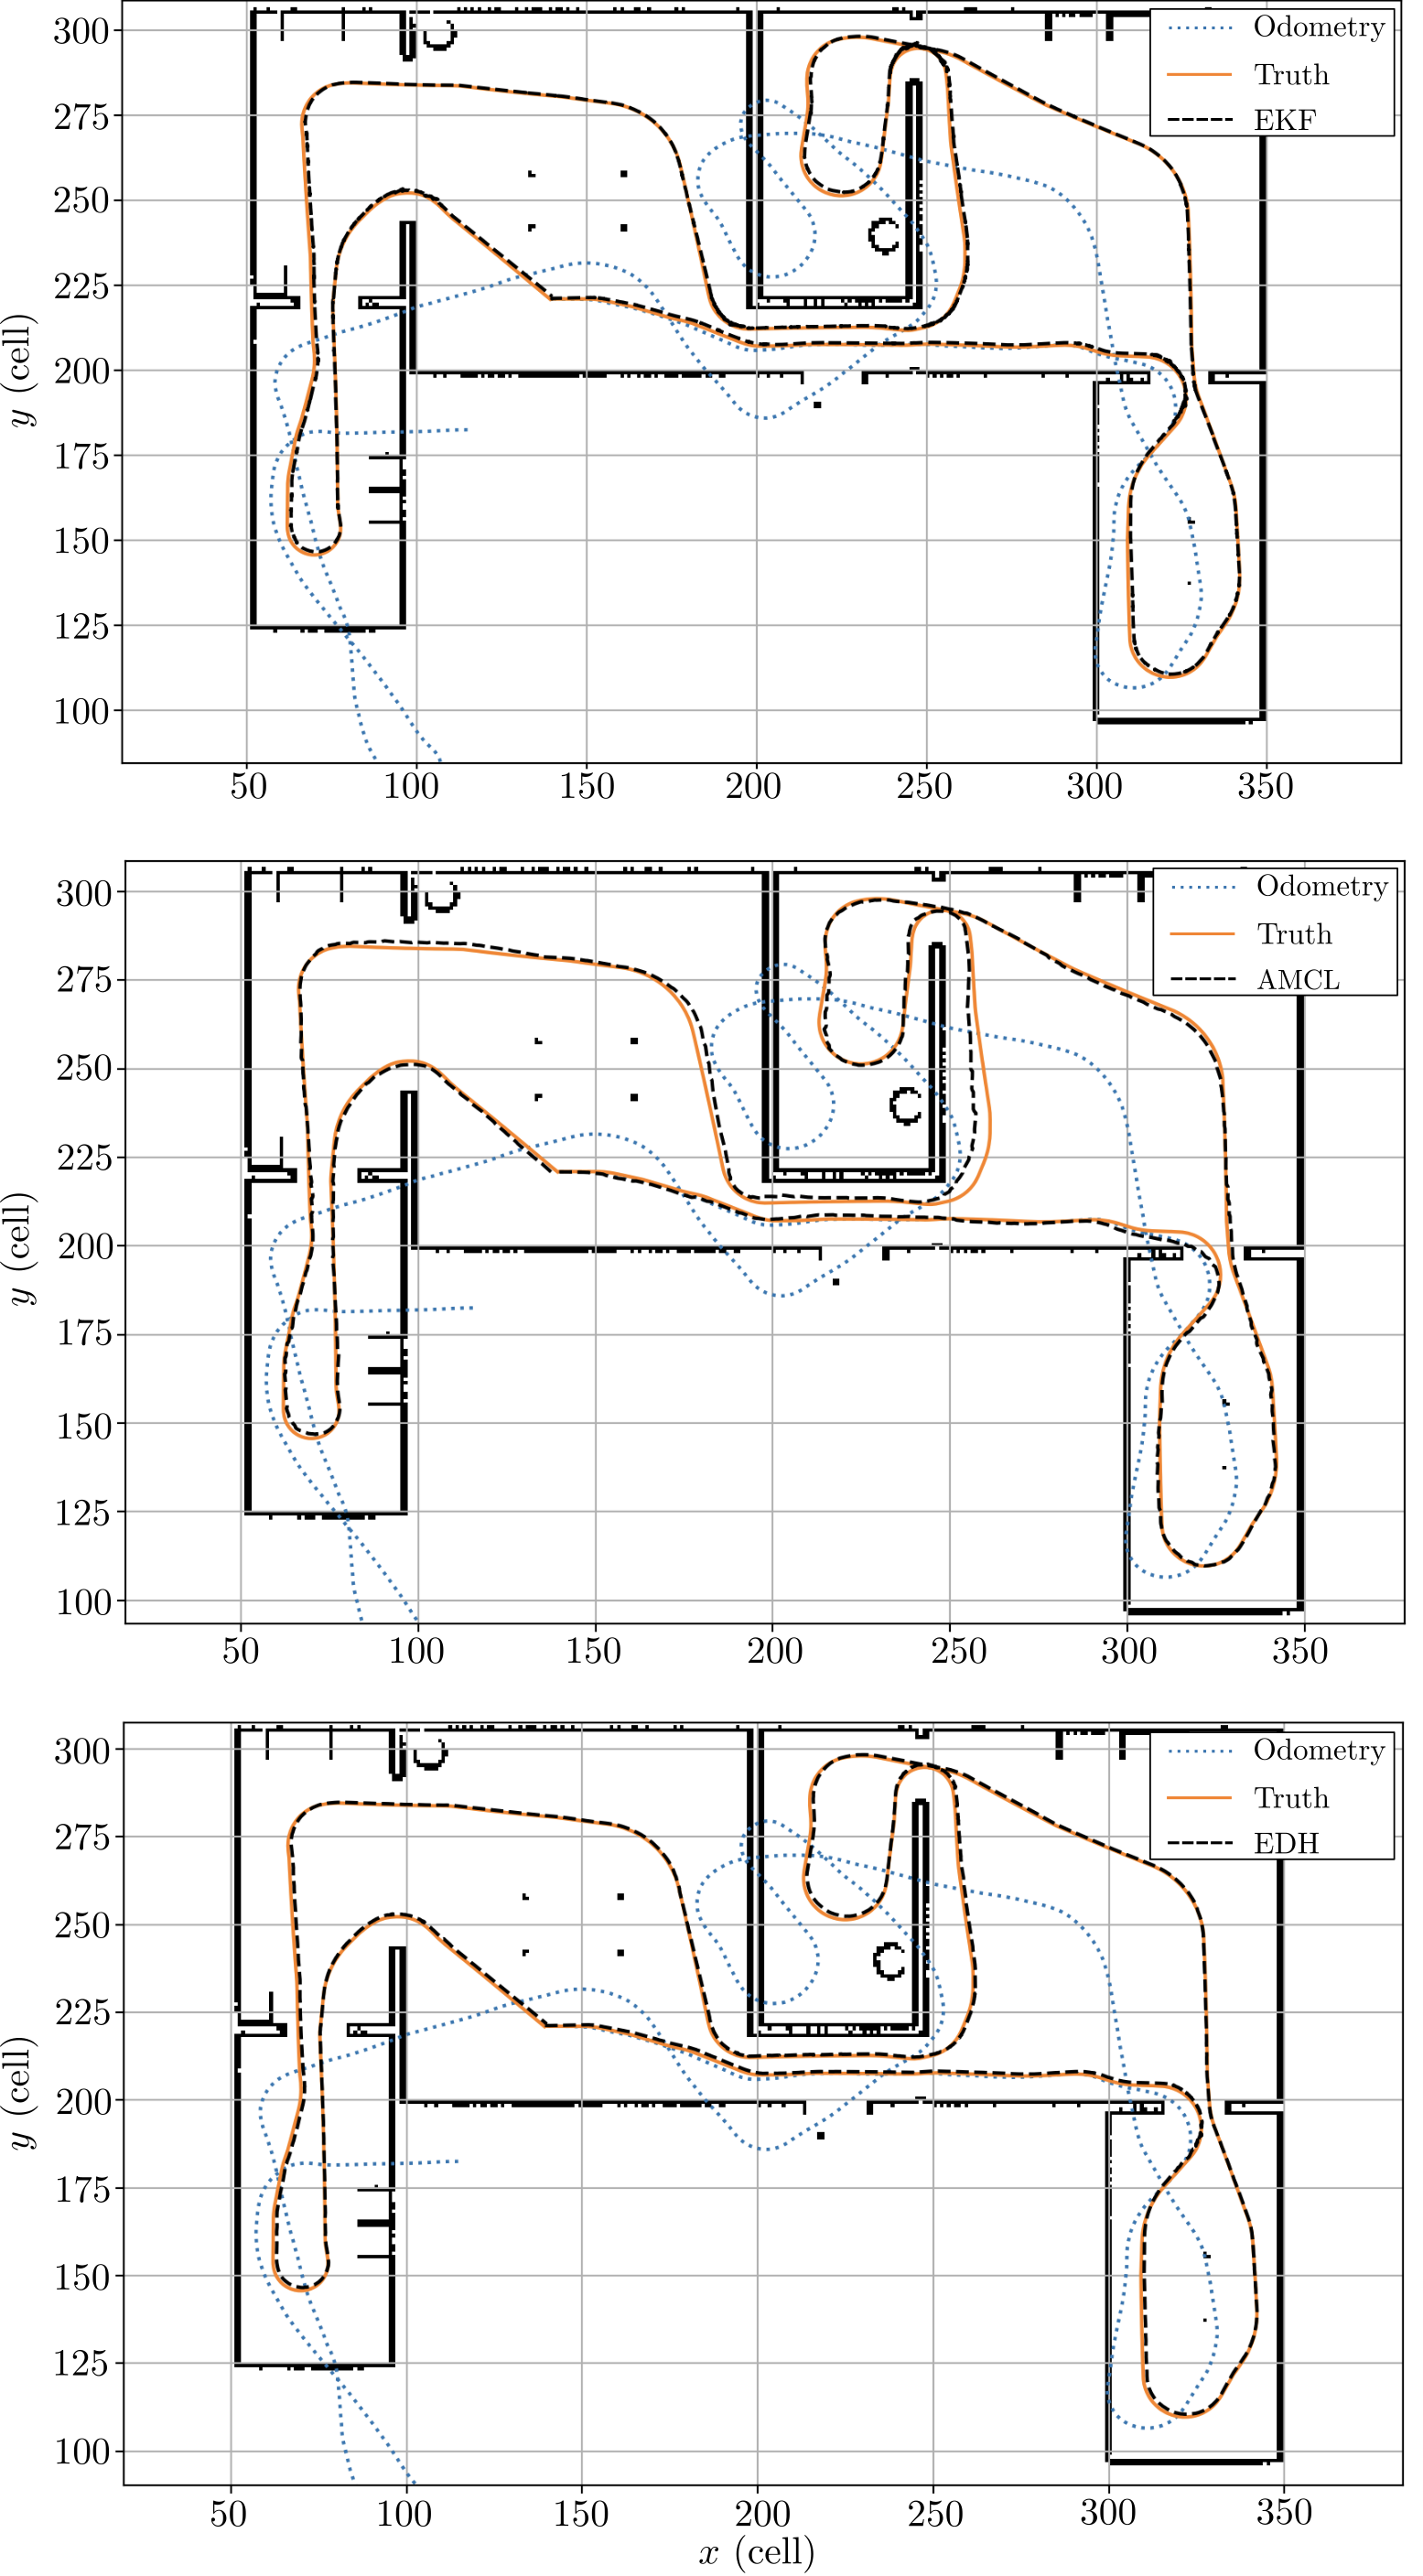
\includegraphics{filtered-tracks.png}
    \caption{Estimated trajectories by the three localization algorithms for $\kappa = 10^{-4}$.}
    \label{fig:filtered-traj}
\end{figure}
